\section{Results}


\textbf{General Benchmark.} Table \ref{tab:tuned-benchmark} shows the experiment results. Without the SOT module, models average 87\% accuracy on the \texttt{TM} dataset and 66\% on the \texttt{SP} dataset, demonstrating their ability to learn from limited samples. 
\texttt{MAML} and \texttt{B} are the top performers across datasets, whereas \texttt{B++} performs worst out of all methods.

% With the SOT module the average accuracy on both datasets increases to 93\% on \texttt{TM} and 83\% on \texttt{SP}. This enhancement, however, is not uniform. Meta-learners significantly benefit, with their performance jumping to 99\% accuracy, showing an average increase of 12 percentage points on \texttt{TM} and 48 percentage points on \texttt{SP}. In contrast, non-meta-learners do not gain from the SOT module, with \texttt{B}'s performance declining and \texttt{B++}'s remaining static.


\begin{table}[ht]
\caption{
    \textbf{Benchmark Results.} Test accuracy of all methods on \texttt{TM} and \texttt{SP} in the 5-way-5-shot setting. We depict the average accuracy and the 95\% confidence interval both without (left) and with SOT (right) and the difference.
    \vspace{5pt}
}

\label{tab:tuned-benchmark}
\centering
\begin{tabular}{llllr}
\toprule
 &  & \multicolumn{2}{@{}c}{\textbf{Test Acc. (\%)}} & \\
 &  & w/o SOT & w/ SOT & Diff \\
\midrule
\multirow[c]{5}{*}{\texttt{TM}} & B & $90.7 \pm 0.7$ & $86.3 \pm 0.9$ & {\color{red} +4.8} \\
 & B++ & $81.9 \pm 0.9$ & $82.8 \pm 0.9$ &  {\color{teal} +1.1} \\
 & MAML & $\mathbf{92.8} \pm 0.5$ & $99.2 \pm 0.1$ & {\color{teal} +6.9} \\
 & MN & $84.6 \pm 0.8$ & $\mathbf{99.7} \pm 0.1$ &  {\color{teal} +17.9} \\
 & PN & $87.1 \pm 0.8$ & $98.6 \pm 0.2$ & {\color{teal} +13.2} \\
\midrule
\multirow[c]{5}{*}{\texttt{SP}} & B & $\mathbf{69.2} \pm 0.7$ & $55.7 \pm 0.8$ & {\color{red} -19.6} \\
 & B++ & $64.1 \pm 0.7$ & $64.6 \pm 0.7$ & {\color{teal} +0.8} \\
 & MAML & $68.7 \pm 0.7$ & $98.0 \pm 0.2$ & {\color{teal} +42.8} \\
 & MN & $68.2 \pm 0.8$ & $\mathbf{99.8} \pm 0.1$ & {\color{teal} +46.5} \\
 & PN & $63.5 \pm 0.7$ & $99.2 \pm 0.1$ & {\color{teal} +56.1} \\
\bottomrule
\end{tabular}
\end{table}
% \caption{
%     \textbf{Benchmark Results.} Test accuracy of all methods on \texttt{TM} and \texttt{SP} in the 5-way-5-shot setting. We depict the average accuracy and the 95\% confidence interval both without (left) and with SOT (right) and the difference.
%     \vspace{5pt}
% }


\textbf{Way-Shot Analysis.} Figure \ref{fig:way-shot} presents the way-shot analysis results for \texttt{PN} on the \texttt{TM} dataset, with and without the SOT module. 
The left subplot shows test accuracy against the number of classes, and the right subplot against the number of samples per class.

Without the SOT module, there's a predictable trend: accuracy decreases with more classes but increases with additional samples per class. 
% However, this pattern changes with the SOT module. Here, accuracy remains stable regardless of the number of ways or shots. Remarkably, in challenging scenarios like 10-way-1-shot, 
% the model sustains a high test accuracy of around 97\%.

\begin{figure}[h!]
    \centering
    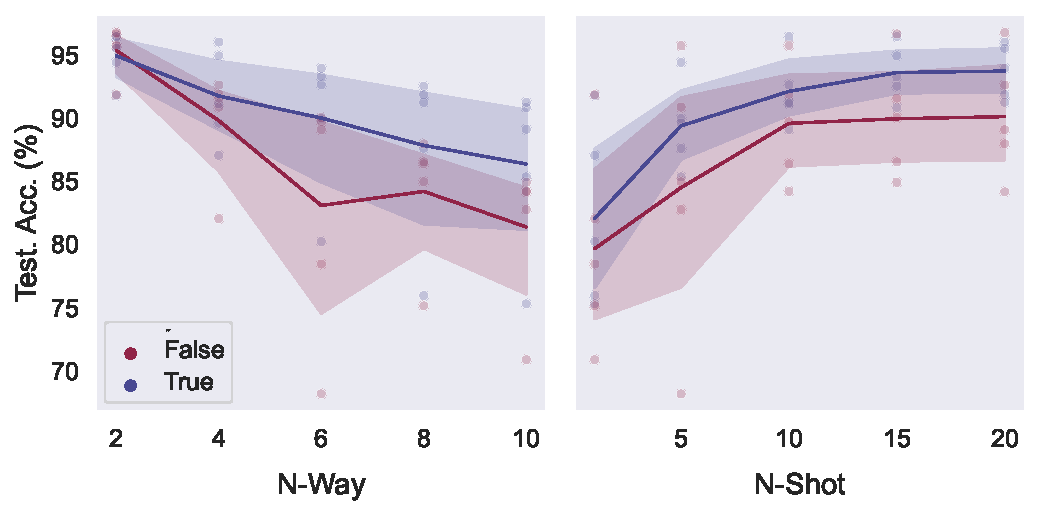
\includegraphics[width=1\columnwidth]{figures/way-shot.pdf}
    \caption{\textbf{Way-Shot Analysis.} Test accuracy of \texttt{PN} on the \texttt{TM} dataset with and without the SOT module in various 
    few-shot learning settings for fixed n-way (left) and n-shot (right). Individual points represent a single experiment. We show the regression line with a 
    95\% confidence interval.}
    \label{fig:way-shot}
\end{figure}
